%% For double-blind review submission, w/o CCS and ACM Reference (max submission space)
\documentclass[sigplan,10pt,review,anonymous]{acmart}
\settopmatter{printfolios=true,printccs=false,printacmref=false}
%% For double-blind review submission, w/ CCS and ACM Reference
%\documentclass[sigplan,review,anonymous]{acmart}\settopmatter{printfolios=true}
%% For single-blind review submission, w/o CCS and ACM Reference (max submission space)
%\documentclass[sigplan,review]{acmart}\settopmatter{printfolios=true,printccs=false,printacmref=false}
%% For single-blind review submission, w/ CCS and ACM Reference
%\documentclass[sigplan,review]{acmart}\settopmatter{printfolios=true}
%% For final camera-ready submission, w/ required CCS and ACM Reference
%\documentclass[sigplan]{acmart}\settopmatter{}

\usepackage{enumitem}
\usepackage{booktabs}
\usepackage{amssymb}
\usepackage{soul}
\usepackage{xspace}
\usepackage{color}
\usepackage{xcolor}
\usepackage{upquote}
\usepackage{listings}
\usepackage{amsmath}
\usepackage{cleveref}

\captionsetup[figure]{font=footnotesize,name={Fig.},labelfont={bf, footnotesize}}
\captionsetup[table]{font=footnotesize,name={Tab.},labelfont={bf, footnotesize}, skip=2pt, aboveskip=2pt}
\captionsetup{font=footnotesize,labelfont={bf, footnotesize}, belowskip=2pt}

\newcommand{\eg}{{\em e.g.}, }
\newcommand{\ie}{{\em i.e.}, }
\newcommand{\etc}{{\em etc.}\xspace}
\newcommand{\vs}{{\em vs.} }
\newcommand{\cmpn}{compartmentalization} 
\newcommand{\heading}[1]{\vspace{4pt}\noindent\textbf{#1}\enspace}
\newcommand{\ttt}[1]{\texttt{\small #1}}
\newcommand{\ttiny}[1]{\texttt{\scriptsize #1}}
\newcommand{\spol}[1]{\scriptsize{\sc#1}}
\newcommand{\pol}[1]{\texttt{\small {\color{purple}#1}}}
\newcommand{\rf}[1]{\ref{#1}}
\newcommand{\wka}{\ttt{a\textsubscript{1}}}
\newcommand{\wkq}{\ttt{q\textsubscript{1-4}}}

% For comments
\newcommand{\eat}[1]{}
\newcommand{\TODO}[1]{\hl{\textbf{TODO:} #1}\xspace}
\newcommand{\todo}[1]{\hl{#1}\xspace}
\newcommand{\nv}[1]{[{\color{cyan}#1 --- Nikos}]}
\newcommand{\kk}[1]{[{\color{magenta}#1 --- kk}]}
\newcommand{\review}[1]{{\color{red}#1}}

\definecolor{editorGray}{rgb}{0.95, 0.95, 0.95}
\definecolor{editorOcher}{rgb}{1, 0.5, 0} % #FF7F00 -> rgb(239, 169, 0)
\definecolor{editorGreen}{rgb}{0, 0.5, 0} % #007C00 -> rgb(0, 124, 0)

\definecolor{cdb}{rgb}{0.37, 0.62, 0.63} % cadet blue

\lstdefinelanguage{sh}{
  morekeywords={for, in, do, done, \|},
  keywordstyle=\color{purple}\ttfamily,
  % ndkeywords={curl, grep, wget, awk, xargs, find, nc, mdc, gunzip, cut, sort, head, join},
  ndkeywordstyle=\color{black}\ttfamily\bfseries,
  identifierstyle=\color{black},
  sensitive=false,
  comment=[l]{\#},
  commentstyle=\color{lightgray},
% morecomment=[s]{/\\*\\*, \\*/},
  stringstyle=\color{darkgray}\ttfamily,
  morestring=[b]',
  morestring=[b]",
% numbersep=1pt,
% numberstyle=\footnotesize\bf\color{gray},   % the style that is used for the line-numbers
  abovecaptionskip=0pt,
  aboveskip=0pt,
  belowcaptionskip=0pt,
  belowskip=0pt,
  frame=none                     % adds a frame around the code
% moredelim=[s][\color{gray}]{c:}{>},
% moredelim=[s][\color{orange}]{/*}{/}
}

\lstset{ %
  backgroundcolor=\color{white},   % choose the background color; you must add \usepackage{color} or \usepackage{xcolor}
  basicstyle=\small\ttfamily,  % the size of the fonts that are used for the code
  upquote=true,
  captionpos=b,                    % sets the caption-position to bottom
% frame=B,                    % adds a frame around the code
  numbers=left,                    % where to put the line-numbers; possible values are (none, left, right)
  numbersep=2pt,                   % how far the line-numbers are from the code
  numberstyle=\tiny\color{gray},   % the style that is used for the line-numbers
  rulecolor=\color{black},         % if not set, the frame-color may be changed on line-breaks within not-black text (e.g. comments (green here))
  framerule=0pt,
	xleftmargin=0pt,
	xrightmargin=0pt,
	breakindent=0pt,
  aboveskip=0pt,
  framesep=0pt,
  abovecaptionskip=0pt,
  aboveskip=0pt,
  belowcaptionskip=0pt,
  belowskip=0pt,
  frame=none,
  framexbottommargin=0pt,
  resetmargins=true
}



%% Conference information
%% Supplied to authors by publisher for camera-ready submission;
%% use defaults for review submission.
\acmConference[PL'18]{ACM SIGPLAN Conference on Programming Languages}{January 01--03, 2018}{New York, NY, USA}
\acmYear{2018}
\acmISBN{} % \acmISBN{978-x-xxxx-xxxx-x/YY/MM}
\acmDOI{} % \acmDOI{10.1145/nnnnnnn.nnnnnnn}
\startPage{1}

%% Copyright information
%% Supplied to authors (based on authors' rights management selection;
%% see authors.acm.org) by publisher for camera-ready submission;
%% use 'none' for review submission.
\setcopyright{none}
%\setcopyright{acmcopyright}
%\setcopyright{acmlicensed}
%\setcopyright{rightsretained}
%\copyrightyear{2018}           %% If different from \acmYear

%% Bibliography style
\bibliographystyle{ACM-Reference-Format}
%% Citation style
%\citestyle{acmauthoryear}  %% For author/year citations
%\citestyle{acmnumeric}     %% For numeric citations
%\setcitestyle{nosort}      %% With 'acmnumeric', to disable automatic
                            %% sorting of references within a single citation;
                            %% e.g., \cite{Smith99,Carpenter05,Baker12}
                            %% rendered as [14,5,2] rather than [2,5,14].
%\setcitesyle{nocompress}   %% With 'acmnumeric', to disable automatic
                            %% compression of sequential references within a
                            %% single citation;
                            %% e.g., \cite{Baker12,Baker14,Baker16}
                            %% rendered as [2,3,4] rather than [2-4].


%%%%%%%%%%%%%%%%%%%%%%%%%%%%%%%%%%%%%%%%%%%%%%%%%%%%%%%%%%%%%%%%%%%%%%
%% Note: Authors migrating a paper from traditional SIGPLAN
%% proceedings format to PACMPL format must update the
%% '\documentclass' and topmatter commands above; see
%% 'acmart-pacmpl-template.tex'.
%%%%%%%%%%%%%%%%%%%%%%%%%%%%%%%%%%%%%%%%%%%%%%%%%%%%%%%%%%%%%%%%%%%%%%


%% Some recommended packages.
\usepackage{booktabs}   %% For formal tables:
                        %% http://ctan.org/pkg/booktabs
\usepackage{subcaption} %% For complex figures with subfigures/subcaptions
                        %% http://ctan.org/pkg/subcaption


\begin{document}

%% Title information
\title{Distribution-oblivious Programming with Dish}         %% [Short Title] is optional;
% \titlenote{with title note}             %% \titlenote is optional;
%                                         %% can be repeated if necessary;
%                                         %% contents suppressed with 'anonymous'
% \subtitle{Subtitle}                     %% \subtitle is optional
% \subtitlenote{with subtitle note}       %% \subtitlenote is optional;
                                        %% can be repeated if necessary;
                                        %% contents suppressed with 'anonymous'


%% Author information
%% Contents and number of authors suppressed with 'anonymous'.
%% Each author should be introduced by \author, followed by
%% \authornote (optional), \orcid (optional), \affiliation, and
%% \email.
%% An author may have multiple affiliations and/or emails; repeat the
%% appropriate command.
%% Many elements are not rendered, but should be provided for metadata
%% extraction tools.

%% Author with single affiliation.
\author{First1 Last1}
\authornote{with author1 note}          %% \authornote is optional;
                                        %% can be repeated if necessary
\orcid{nnnn-nnnn-nnnn-nnnn}             %% \orcid is optional
\affiliation{
  \position{Position1}
  \department{Department1}              %% \department is recommended
  \institution{Institution1}            %% \institution is required
  \streetaddress{Street1 Address1}
  \city{City1}
  \state{State1}
  \postcode{Post-Code1}
  \country{Country1}                    %% \country is recommended
}
\email{first1.last1@inst1.edu}          %% \email is recommended

%% Author with two affiliations and emails.
\author{First2 Last2}
\authornote{with author2 note}          %% \authornote is optional;
                                        %% can be repeated if necessary
\orcid{nnnn-nnnn-nnnn-nnnn}             %% \orcid is optional
\affiliation{
  \position{Position2a}
  \department{Department2a}             %% \department is recommended
  \institution{Institution2a}           %% \institution is required
  \streetaddress{Street2a Address2a}
  \city{City2a}
  \state{State2a}
  \postcode{Post-Code2a}
  \country{Country2a}                   %% \country is recommended
}
\email{first2.last2@inst2a.com}         %% \email is recommended
\affiliation{
  \position{Position2b}
  \department{Department2b}             %% \department is recommended
  \institution{Institution2b}           %% \institution is required
  \streetaddress{Street3b Address2b}
  \city{City2b}
  \state{State2b}
  \postcode{Post-Code2b}
  \country{Country2b}                   %% \country is recommended
}
\email{first2.last2@inst2b.org}         %% \email is recommended

\newcommand{\cf}[1]{(\emph{Cf}.\S\ref{#1})}
\newcommand{\sx}[1]{(\S\ref{#1})}
\newcommand{\sys}{{\scshape Dish}\xspace}
\newcommand{\unix}{{\scshape Unix}\xspace}

\setlist{noitemsep,leftmargin=10pt,topsep=2pt,parsep=2pt,partopsep=2pt}

%% Abstract
%% Note: \begin{abstract}...\end{abstract} environment must come
%% before \maketitle command
\begin{abstract}
  \nv{placeholder}
  Distributed systems offer notable benefits over centralized ones.
  Reaping these benefits, however, requires programming in a way that makes distribution explicit---\eg via new programming languages, distributed framework interfaces, or distribution annotations.
% 
%   \emph{Distribution-oblivious programming} is a new approach for..?
  This paper presents \sys, a shell variant that automatically and correctly scales out distribution-oblivious shell pipelines. %  with regards to the sequential program.
  % leveraging the insight that such programs already express stream computations, with their stages falling under a few, known distributability classes.
  \sys's insight is that shell pipelines already express stream computations that can automatically distributed.
  To achieve this, \sys
% a series of techniques for automatically 
decomposes primitives into distributability classes,
identifies high-distributability stages,
applies rewriting rules for largest possible subprograms,
and orchestrates the distributed program.
Its runtime component provides orchestration and planning support during the execution of the program.
% 
% Key challenges include 
% surprisingly expressive, 
% maximally distributable subprograms
% 
Experiments for complex pipelines show substantial speedups and the ability to operate on large input datasets, all without any developer input.
\end{abstract}


%% 2012 ACM Computing Classification System (CSS) concepts
%% Generate at 'http://dl.acm.org/ccs/ccs.cfm'.
\begin{CCSXML}
<ccs2012>
<concept>
<concept_id>10011007.10011006.10011008</concept_id>
<concept_desc>Software and its engineering~General programming languages</concept_desc>
<concept_significance>500</concept_significance>
</concept>
<concept>
<concept_id>10003456.10003457.10003521.10003525</concept_id>
<concept_desc>Social and professional topics~History of programming languages</concept_desc>
<concept_significance>300</concept_significance>
</concept>
</ccs2012>
\end{CCSXML}

\ccsdesc[500]{Software and its engineering~General programming languages}
\ccsdesc[300]{Social and professional topics~History of programming languages}
%% End of generated code


%% Keywords
%% comma separated list
% \keywords{keyword1, keyword2, keyword3}  %% \keywords are mandatory in final camera-ready submission


%% \maketitle
%% Note: \maketitle command must come after title commands, author
%% commands, abstract environment, Computing Classification System
%% environment and commands, and keywords command.
\maketitle


\section{Introduction}

% 1. Shell scripting; pipelines, in particular, are a common abstraction for expressing filters
% They are an easy way to , because they combine a set of assumptions that work well with Unix
% They work great on a single machine, but are difficult to scale out
% Could we fully automate distribution? 
% The key insight is that pipelines already express a domain-specific
% computation that is easily amenable to distribution.
% 

Distributed systems offer significant benefits over their centralized counterparts---for example, they can speed up expensive computations or process data that would not fit into any single machine.
% offer notable benefits over their centralized counterparts:
%   using partitioning and replication, they can process and store data with increased throughput and fault-tolerance.
% Yet, only a minority of developers, employed by the select few companies that deal with massive datasets, have the luxury of engineering software systems with distribution baked in from the start.
% The remaining majority starts by developing and deploying software in a centralized manner---that is, \emph{until} there is a significant change of requirements, such as a load increase.
Despite these benefits, their development remains different from and significantly more difficult than their centralized counterparts.
Whereas anyone can quickly stitch together a Bash script to compute on a single computer, 
  % domain-experts routinely glue scripts together to process and share data. % without the help of a computing expert.
   scaling out to multiple ones requires expert labor around ``point'' solutions with expensive setups, restricted programming interfaces, and exorbitant composition costs~\cite{taurus:14, dios:13, andromeda:15, pywren:17, futuredata:18, nefele:18}.

To understand this sharp contrast, consider calculating term frequencies over a set of input files:

% \begin{lstlisting}[language=sh,float=h,numbers=none]
% cat doc.ms |                   # print input file
% groff -t -e -mandoc -Tascii |  # remove formatting
% col -bx |                      # remove backspaces 
% tr A-Z a-z |                   # convert to lower case
% tr -d '[:punct:]' |            # remove punctuation
% sort |                         # put words in alphabetical order
% unique |                       # remove duplicate words
% comm -13 /usr/share/dict -     # report words not in dictionary 
% \end{lstlisting}

\begin{lstlisting}[language=sh, float=h, numbers=none, escapeinside={($}{$)}]
cat * | tr -cs A-Za-z\n | tr A-Z a-z |    ($$[p_1]$$)
  sort | uniq -c | sort -rn | head 5 > out
\end{lstlisting}

\noindent
Program $p_1$ creates a character stream, breaks it into words, transliterates to lower-case, sorts to group duplicates, summarizes them with a counter, sorts them in descending order, picks the top five results and writes them to a file \ttt{out}.
Combining several features, \unix makes small tasks easy to express;
  for a user with \emph{one} computer and small input, this pipeline takes a few seconds to compose and execute~\cite{bentley1986literate}.
% composition allows the composition of general primitives

% Key insight 
% % The garden-hose philosophy is similar to Haskell 
% This pipeline takes an input file (line 1), removes 
% * do not need to use specialized frameworks for composition---instead, as long as they conform to the shell, individual primitives can be written in any programming language.
% * do not need to rewrite ---

\begin{figure}[t]
\centering
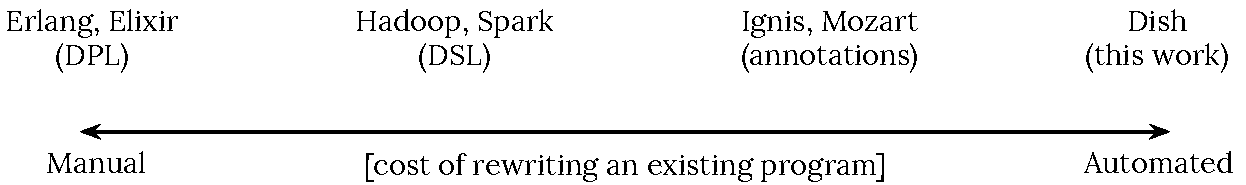
\includegraphics[width=0.49\textwidth]{./figs/dish_spectrum.pdf}
\caption{
  \textbf{Cost of Manual Effort.}
	\sys sits at the automation end of the spectrum, automatically distributing shell pipelines while maintaining their correctness. A more complete picture is presented in the related-work section~\sx{rt}.
}
\label{fig:spectrum}
\end{figure}


%      dish      ignis, mozart    hadoop, spark, ...      erlang, elixir
%       \/           \   /             \     /                \   /
% auto <-------------------------------------------------------------> manual
%                      [rewrite (not write) cost]

For a user with many computers and larger inputs, however, developing $p_1$'s distributed equivalent requires a significant effort.
% The scope of such rewrites, and therefore the cost of manual effort, can vary considerably.
For simple pipelines that capture in restricted models of computation, this effort amounts to expressing the computation using the primitives provided by a big-data framework~\cite{mapreduce:08, ciel:11, spark:12, naiad:13} or domain-specific language~\cite{alvaro2011consistency, distal:13, meiklejohn2015lasp}---an unjustifiable cost for one-off pipelines that take a few minutes to compose (but are applied to large datasets).
More complex pipelines, such as the ones presented in later sections, require full-fledged distributed programming language~\cite{erlang:96, lopes1997d, acute:05, mace:07, cloudhaskell:11, ScalaLoci:18}. %  or a distributed operating system---\eg Plan9's \ttt{rc} shell.
In these cases, manual rewriting is expensive and can introduce new bugs, cascading changes, or divergence from legacy functionality.
Could the generation and execution of $p_1$'s distributed version be fully and correctly automated?

% Some (parts of) pipelines require only moderate effort, as they are 
% For some pipelines, this effort is merely moderate, as 
%  can be expressed in domain-specific frameworks---for example, Hadoop and Spark provide a few purely functional primitives that 
%   ---still requiring rewriting the program in a different (\eg Scala for Spark).
% 
% This effort is moderate if the program expressed by these pipelines fits into a domain-specific framework.
% At times, such pipelines
% As long as the program fits into the model this is only moderately difficult;
% 
% For many legacy pipelines  
%  has to choose between three options, all of which require significant manual effort.
% The most invasive is to rewrite the entire program in a distributed programming language
% The most popular is to leverage 
% 
% Use a distributed programming language, even higher rewrites
% Or use some form of annotations 
% 
%  this requires rewriting portions of the program in a new language and use operations
% 
% 
% In the simplest case, annotations
% 
% Often, they only focus on a few parts of the system---for example, upgrading to a distributed storage layer.
% More rarely, companies rewrite entire systems (\eg Twitter's Ruby-to-Scala rewrite~\cite{twitter}), a process that is notoriously difficult under schedule constraints and competitive pressures~\cite{rewrite1, rewrite2}.
%  especially since software today makes extensive use of third-party modules~\cite{breakapp:plos:2017}.
% 

% If developers have already expressed their computation as a Unix pipeline, they should not have to manually rewrite the program in other environment---\eg Hadoop, Spark---to exploit distribution.


The key insight behind \sys is that the language of the Unix shell already encodes stream processing, providing most of the information required for distributing a computation.
\sys builds on this insight with a careful study of the scalability properties of shell primitives and its commands, paired with a novel rewriting scheme that identifies maximal pipeline sub-expressions that are candidates for scale-out.
We term the result \emph{distribution-oblivious programming}---a series of techniques that fully automates program distribution while provably maintaining correct (non-distributed) semantics.

Key benefits include the ability to scale legacy computations onto
\sys converts legacy shell pipelines into their distributed equivalents fully automatically, offering $100\times$ improvements in performance without a single line of additional code or annotation.
Most importantly, \sys provides an architectural lesson:
  the current design shows that large-scale efforts in the distributed- and operating-system literature to provide a \unix-like distributed equivalent could have been simplified by a thin (but sophisticated) rewriting shim like the one \sys provides.

% % Make Unix benefits explicit?
% Indeed, the primary reason behind $p_1$'s succinctness is that the pipeline is a domain-specific language for describing operations over streams.
% Key elements of \unix are the ability to compose programs written in different languages, the abstraction of a file system as a set of resident streams, a small but extensible library of commands, and the ability to resolve names within a global context.
% Under the hood, the \unix kernel buffers results, synchronizes processing stages, and generally orchestrates the computation.

% Primitives 
% \sys enables \emph{distribution-oblivious programming}: 
%   multi-order of magnitude speedups with correctness guarantees and without any developer effort.
% 
% The a series of transformations that 
% Second, we are using describing composition . For this, we are restricting the study to a subset of the POSIX shell--
% 
% Local operations and identifiers have to be carefully translated to distributed ones, a translation that depends on the types of the operations and associated identifiers.
% 
% The semantics is enough to capture powerful features such as stream branching and feedback constructs found in practice and in the system's evaluation.

The paper is structured as follows.
We first start with a background section outlining pipeline concepts~\sx{bg}.
Sections \ref{classes}--\ref{recipes} highlight our key contributions:\footnote{
  This is not precise, we'll need to wait until it matures a bit.
}
\begin{itemize}

  \item
  \S\ref{classes} overviews \sys and introduces several scalability and distributability classes.

  \item
  \S\ref{rewrite} presents a set of rewriting transformations for identifying maximal pipeline sub-expressions, candidates for scale-out.

  \item
  \S\ref{other} details other concerns, such as distributed state management and extensibility.
\end{itemize}

\noindent
\sys's evaluation~\sx{eval} uses a combination of one-liner micro-benchmarks that highlight certain features and three multi-line macro-benchmarks---a web crawling and indexing engine, a production genomics pipeline, and a large-scale weather analysis.
We close with a discussion of related prior work~\sx{related} and possible future directions~\sx{discussion}.

\begin{figure*}[t]
\centering
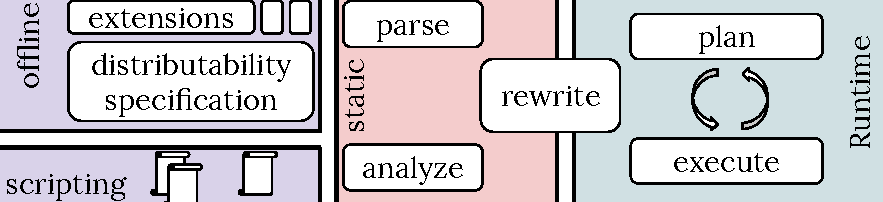
\includegraphics[width=0.49\textwidth]{./figs/dish_overview.pdf}
\caption{
  \textbf{Applying \sys to $p_1$.}
}
\label{fig:example}
\end{figure*}


\section{Background}
\label{bg}

This section breaks down $p_1$ to presents important background on and challenges
of shell scripting.

\subsection{Unix Pipelines, Informally}
\label{bg:pipelines}

Pipelines are a mechanism for program composition.
Individual programs, specified as commands, conform to a common but general interface. 
For now, this interface allows a combination of the following:
  accepting input from the standard input stream (stdin),
  generating output to the standard output stream (stdout), and
  generating errors or diagnostics to the standard error stream (stderr)
Standard streams are streams of characters with a few special characters---for example, EOF is a special end-of-file character signaling the end of the input stream.
% For Unix commands, the newline character is special; as such, Unix streams can be seen as lazy lists of strings---lines of text separated by the newline character.

Leveraging this interface, pipelines chain together commands by their standard streams, such that the output stream of one command (stdout) is passed directly as input (stdin) to the next one.
Pipeline chaining goes hand-in-hand with the Unix toolbox philosophy: 
  programs do one thing well, they work together, and they manipulate text streams as their universal interface.
The next few paragraphs describe the details.


\heading{Basics}
The standard shell syntax for pipelines a list of commands separated by vertical bars (``pipes'', in Unix terminology).

that are not interpreted by the shell, but are local to each command.

Additional details augment this simple interface.
Commands can be specified with options arguments

\begin{figure}[t]
\centering
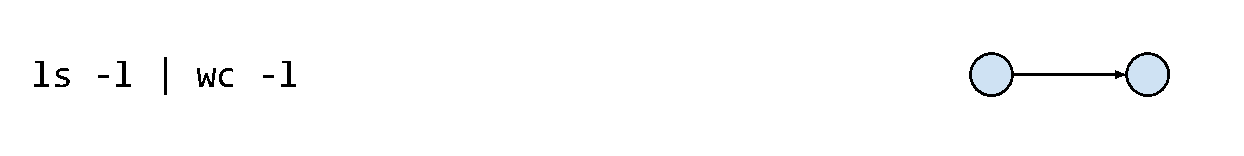
\includegraphics[width=0.45\textwidth]{./figs/dish_ex1.pdf}
\label{fig:example}
\end{figure}


\begin{lstlisting}[language=sh, float=h, numbers=none, escapeinside={($}{$)}]
 ls -l | wc -l                           (($$p_2$$))
\end{lstlisting}

\heading{Generation}
A central concept in pipelines---and Unix, in general---is the file system, which allows interfacing with persistent data.
There are many commands that take as input a file identifier 
Reading a file or a set of files generates a stream; 
  similarly, streams can be trivially redirected to the file system---by appending with the file identifier.

Expansion---the key is that expansion and evaluation are handled by the shell at an earlier stage 
The most powerful---and interesting, for \ttt{dish}---type of expansion is subshell expansion, that allows replacing entire input streams 


\begin{lstlisting}[language=sh, float=h, numbers=none, escapeinside={($}{$)}]
 cat * | wc -l > out.txt                 (($$p_3$$))
\end{lstlisting}

\heading{Identifiers}

\kk{We have to mention character vs line based parallelism somewhere,
  and that we choose to see lines as the data quantum}

The file-system is a common abstraction layer used for many other operations than just serving files (this will be become clearer when talking about file-system commands in \S\ref{bg:cmd}).
as such, different identifiers many not resolve to actual files, but rather in-memory or OS-internal structures.

At a high level, POSIX defines several file types:
(-) regular files, storing lines of text or binary data,
(d) directories, grouping together multiple other files,
(l) symbolic links, pointing to other files,
(p) named pipes or FIFOs, communication primitives that can be named and manipulated like files,
(s) domain sockets or DSes, full-duplex communication primitives that support passing file descriptors, and
(b or c) special files, interfaces to device drivers or low-level abstractions, presented as ordinary files.

Most of these identifiers are manipulated by file-system commands---\eg \ttt{mkdir} for directories and \ttt{mkfifo} for FIFOs.
FIFOs and DSes look like files but are streams.

Special files are particularly interesting because they are resolved to OS structures.
One set is pseudo-devices---device files that simply;
For example /dev/urandom returns a stream of random characters and /dev/null accepts and discards all input written to it.
Another set is proc filesystem (procfs), a special filesystem in Unix-like operating systems that presents information about processes and other system information.
For example, /proc/PID/cmdline contains command that originally started the process and /proc/PID/cwd contains a symlink to the current working directory of the process.

sysfs is a pseudo file system provided by the Linux kernel that exports information about various kernel subsystems, hardware devices, and 

/modules, one of the most important files in /proc, containing a list of the kernel modules currently loaded . It gives some indication (not always entirely correct) of dependencies.
/cpuinfo

symbolic links, FIFO specials, 
device files
block special, character special, 
and domain sockets.

There are 3 standard streams (stdin, stdout, stderr) created automatically for most Unix programs.
These correspond to \ttt{/dev/fd/0}.
% These streams are created by the C library (glibc) at the start of program execution,
and new streams can be created to connect to files, sockets, pipes,

Unix already specifies a few classes of files:

Here are a few special files:
  \ttt{proc} called 

Technically, anonymous pipes show up as file identifiers in a hidden filesystem.
Similarly, open files and other ephemeral identifiers 


\begin{lstlisting}[language=sh, float=h, numbers=none, escapeinside={($}{$)}]
 cat /proc/ >                            (($$p_4$$))
\end{lstlisting}

\heading{Stream Manipulation}
A small but powerful set of primitives are concerned with stream manipulation.
First, as described above, several commands can be redirected
Second, 

\ttt{xargs}
\ttt{tee}

In combination, these constructs are powerful enough to introduce circular streams. % or stream cycles?

Explicit Redirection
Implicit splitting and merging 
This can be done through the file-system operators 

\begin{lstlisting}[language=sh, float=h, numbers=none, escapeinside={($}{$)}]
 cat /proc/ >                            (($$p_5$$))
\end{lstlisting}

\heading{Composition}
anonymous pipes

Composition

The shell provides several ways of grouping commands and manipulating their
overall input and output channels 

{ echo 1; echo 2; } > out.txt

\subsection{Comnands}
\label{bg:cmd}

% Sets vs. Classes

Distributability classes, based on how 

\heading{Preliminaries}

\heading{POSIX, GNU Core-utils, and beyond}

\heading{Stateless}

\heading{Pure}

\heading{File-system}

\heading{Side-effectful}

\heading{Irreversably Side-effectful}

\subsection{The Shell Language}
\label{bg:shell}

\heading{Implicits}
Expansion
Implicits
Context

\heading{Language Constructs}

Even without these, the Unix pipeline language is powerful enough to capture complex pipelines.

We can encode powerful

\section{Dish Overview}


\section{Extensibility}

ULTRA DRAFTY:

\kk{Text point: A problem that is specific to the shell is
  extensibility.}

The major characteristic that makes the shell popular and very useful
is its extensibility, as also mentioned in \Cref{bg}. Commands change,
get extended, and each user continuously installs more commands to use
in their system.

\kk{Text point: This restricts the space of solutions for distribution
  of shell scripts}

This means that any one-time solution is not satisfactory, since it
would very easily become obsolete, or it would only handle a limited
amount of shell scripts.

\kk{Text point: The characteristics of a good solution}

A solution that applies to shell programms should thus be extensible,
in the sense that adding or changing a command, doesn't invalidate the
assumptions that the tool makes. In our case, the information about
the command categories. A developer of a new command, should be able
to categorize it accordingly, and succinctly describe how the system
can distribute a command.

\kk{Solution: A lightweight language that can be used by a command
  developer to categorize it for distribution.}

We address this issue by designing a lightweight language whose
purpose is to categorize a command, describes how it reads its input
(meaning in what order), and how to distribute it (in case it is
pure). \kk{I am not sure if the order in which a command reads its
  input will be part of the language since many commands can be made
  to read from one place (like stdin or their first argument). Even in
  that case though, where the command only reads from one argument, we
  have to make sure that there is a way for the user to pinpoint which
  argument does a command read from.}

\subsection{Categorization Language}

\kk{Text point: Introduce problem: Most shell commands, belong to
  different classes depending on their flags, arguments}

Consider the command \texttt{cat} \kk{Maybe that is not he best
  example. TODO: Find a good example of a simple command that is in
  different classes depending on the arguments.}. When used without
any flag it is stateless, etc...

\kk{Text point: Our language must be able to categorize commands to
  different classes according to their arguments.}

\kk{We should have a crisp point about why we have this categorization
  language, and why don't we just allow someone to write a function in
  python for each command, that given the command and its arguments,
  returns whether the command category. Possible arguments include,
  the fact that this language is simpler to use, especially by non
  experts that just run some script but have installed some commands
  that are not ``supported''. Another possible argument is that we
  could be able to reason about the constructs of the categorization
  lagnauge, and that they will be easier to read and
  understand. Another argument is that since these categorizations
  should be shareable among users, it would be bad to execute
  arbitrary python code, so using this language, expressivity is
  limited. All of these arguments are a little bit weak though. Niko,
  what do you think?}

Sketch of the language:

Some kind of lightweight annotation configuration language (like
yaml), that contains a record for each command.

A record contains a sequence of predicates => categories. Each
predicate is a combination of not, or, and and the atomic predicates
are the presence of a flag, or an equality that checks that the value
of a flag is equal to something (because flags can also have
values). The final predicate can be left empty, and it is trivially true.

Interpreter:

Given a command and the set of its arguments, the intepreter returns
the command category. In does so by returning the category of the first
predicate that matches.

\kk{Would it be meaningful to give the syntaxx of the language
  formally?}

\kk{If we talk about the language it would be good to give some
  statistics about how many commands (out of the ones that we have
  classified) can be represented with one, two clauses etc. If we have
  a different solution (like python function that given a command and
  its arguments returns the category) then we could talk about how
  many lines of code it took to categorize all the commands that we
  did.}

As described in distributability\ref{}, the abstract notion of a
program that we have is programs with one input and one output
stream. The command developer must be able to express the input
argument of a commmand (or if it is the stdin).

\kk{Question: Do we need to handle all commands (even the ones that
  could have their input split in several different arguments? or can
  we somehow easily make these ones just take their input from one
  place (e.g. by adding a cat before them).}

\kk{Possible solutions for this (if we have already turned commands
  with more that one input to commands with one input): Have a
  positional reference to the argument that is input (or ``stdin'' if
  it is the stdin). Example: the last argument [-1] of grep is its
  input.}

\kk{It seems that even the arguments might depend on flags (e.g. grep
  checks the current directory if asked recursively, or the stdin
  otherwise), so maybe we should again have a sequence of predicates}


\kk{Note: Since a categorization language will probably not be
  complete (especially the one showing the input arguments) there
  should be a backup mechanism, when the language is not expressive
  enough, like a python function that categorizes the command, and
  returns its input argument if it is stateless.}

\subsection{Pure Commands}

Even though stateless commands are a big percentage of all of them,
there are a lot of useful and popular pure commands.

As mentioned in distributability, pure commands can be broken down
into different categories. We might be able to get ideas about this
from this paper:
\url{http://www.cs.toronto.edu/~azadeh/papers/pldi17-ex.pdf} and its
continuation in PLDI 2019.

Can we find a solution for the commands in coreutils?



\section{Intermediate Representation/Dataflow graph}

\kk{Try to be more formal in the section, by using the notation that
  is defined in the nodes paragraph.}

In order to effectively apply optimizations and distribute a shell
script, it first has to be translated to a manipulable
representation. As mentioned in \ref{}, the two main abstractions of
the shell, are files that contain data, and commands that communicate
through these files. We propose a slight variation of the standard
dataflow graph, that is commonly found in stream processing systems,
as the representation of a distributed shell computation. The main
benefit of the dataflow graph model is that it clearly exposes
operator level parallelism, as different nodes can be independent
processing workers. In our case each node represents a command, and
each edge represents a file.

\kk{Before that I have to mention that the basic data type $D$ is a
  line of characters. If we move the edges section before the nodes
  that will be fine.}

\paragraph{Nodes - Commands}

Nodes $f$ of the graph represent functions from one (possibly empty)
input stream to an output stream $f : D^* \rightarrow D^*$.  This
representation captures the majority of shell commands. The nodes $f$
are monotonic, meaning that they cannot retract their output. More
formally, if $f(x) = y$, then for any $x'$, there exists $y'$ such
that $f(x.x') = y.y'$, where $.$ is standard concatenation and will be
omitted from now on. An example of a node is the following command
\kk{Does it need ref? Also maybe this example is too trivial and can
  be removed.}:

\begin{lstlisting}[language=sh, float=h, numbers=none, escapeinside={($}{$)}]
 grep ``foo''
\end{lstlisting}

\noindent
This command takes a stream of lines from its standard input and
returns a stream of lines on its standard output. An important
observation though is that commands in the shell might read their
input stream from a sequence of different sources. An illustrative
example is the command \kk{Inline listing}cat which reads its input
from a combination of files and its standard input.

\begin{lstlisting}[language=sh, float=h, numbers=none, escapeinside={($}{$)}]
 cat x - y
\end{lstlisting}

\kk{Should I reference that this example was takes from the cat
  manpage?} The example above reads file \texttt{x} until it
encounters the end of file, then reads from \texttt{stdin}, and then
reads from \texttt{y}. In order to handle this particularity, nodes in
the dataflow graph can have many incoming edges, that are clearly
ordered in a sequence. Note that this comes in contrast with standard
dataflow graph representations where multiple incoming edges either
mean zipping the input to pairs, or arbitraliy interleaving the
different inputs.


\kk{A note about nodes and commands that can write and read from more
  files that the ones in their streams}

Note that nodes can read from more files than just the files of their
stream (or respectively write to more files that their output stream),
however these files are static (e.g. used for configuration or logging
\kk{Would an example here help}) and do not represent streams of data,
and therefore are not considered part of the dataflow graph. Because
of the assumption in section Front End \ref{}, that each file exists
only once in the dataflow graph, we can safely assume that reading and
writing to these static files does not interfere with the distributed
implementation, and doesn't alter the behaviour of the program.

\paragraph{Edges - Files}

\kk{Maybe edges has to be moved before nodes, so that we can define
  the line data type}

Edges in the dataflow graph represent files, the basic data
abstraction of the shell. They are used as communication channels
between nodes in the graph, and as the input or output of the whole
graph. Edges are represented as possibly unbounded streams of type
$D*$, where $D$ represents a line, that is a sequence of characters
followed by \verb|\n| \kk{or EOF?}. They could either refer to a
specific named file in the file system, or just be FIFO pipes that
used for interprocess communication \kk{Are there any other file
  types, such as URLs, ...?}.

\kk{Show an example pipe and its graph}.

In order to expose operator parallelism with the output of a command,
files that don't point to a resource can have an upper bound on the
lines that they can tranfer. The following example illustrates why
this is essential.

\kk{An example of a command that has two outputs and one goes to one
  command, while another output goes to a different one. Maybe only
  show the graph here and not the command itself.}

On the other hand, some forms of data parallelism can be exposed when
knowing the size of the input files. As mentioned in \ref{} some pure
commands (such as cat -n) only need line information to become
stateless, and knowing the size of a file could allow the system to
split it in different chunks that can be processed independently. To
account for that, edges that refer to an input resource contain the
number of lines of the file that they refer to. \kk{At the moment this
  is not supported by our real system. The whole paragraph above can
  go if we decide that it is not a good idea to talk about it now.}

Finally, the edges that don't refer to a resource and do not start
from a node in the graph represent the graph input, while the edges
that don't refer to a resource and do not point to a node in the graph
are its outputs.

\kk{(Maybe) Depending on which of the two paragraphs goes last
  (nodes/edges), I have to explain there that the last incoming edge
  to a node must be unbounded (if it doesn't point to a resource). I
  am actually not sure whether I should include this here.}


\kk{(Maybe) It might be beneficial to mention that many inputs do not
  represent the same thing as many outputs. These two notions are not
  symmetric.}

\paragraph{Merge and Split}

\kk{Mergers and splitters, and how they are implemented using shell
  constructs (cat and head). This subsection might be a better fit in
  some other section, maybe something related to the planner or the
  implementation, as it is a very elegant way to implement splitters
  and mergers while staying completely inside the shell programming
  model.}

It is common in the dataflow graph for a node to have many incoming
edges, or many outgoing edges (when all but the last outgoing edges
are bounded). However some nodes, might read their input from one file
(e.g. stdin). In this case, the distributed implementation needs to
concatenate input files, and split output files. Here is an example:

\kk{Show an example graph! of cat | tr | sort. The command in the
  middle must only take input from one file (maybe just stdin).}

\kk{This transition needs to be stronger} Luckily, the shell offers
primitives for file manipulations that can be used to implement a
merger and a splitter. More concretely a merger can be implemented by
a simple \verb|cat|. Given a set of input files \verb|in1, in2, ...|
and an output file \verb|out|, a merger can be implemented as:

\begin{lstlisting}[language=sh, float=h, numbers=none]
 cat $in1 $in2 ... > $out
\end{lstlisting}

\noindent
On the other hand, given an input file \verb|in| that is a FIFO pipe,
and two output files \verb|out1, out2| the first of which is bounded
to \verb|N| lines, a 2-splitter can be implemented as:

\begin{lstlisting}[language=sh, float=h, numbers=none]
 head -n $N $in > $out1 ; cat $in > $out2
\end{lstlisting}

\noindent
Using the 2-splitter as a building block, a pipe can be split to
arbitrarily many different pipes.

\kk{Do I also need to include a splitter for normal files?}


\kk{Intermediate Representation Section notes:}

\kk{Explain how the assumptions made in the front end give as
  correct/safe operator level parallelism. Maybe this must go in the
  Front-end section.}



\section{Front End}

\kk{Maybe this becomes a subsection either in the intermediate
  representation or in the planner.}

We parse a shell script using a posix compliant parser that returns
the ast.

\kk{Text point: The AST Is not a very good data structure to
  manipulate for distribution, so we translate it to a kind of a
  dataflow graph.}

\subsection{Distributable Subtrees}

\kk{Text point: Problem: Not all parts of a shell script are
  distributable, so we cannot arbitrarily distribute. Here we have to
  make our assumptions clear}

Even though commands are split in categories, and several pipelines
are distributable, not all parts of a shell script are stateless and
several of them have effects that could affect the behaviour of a
program after distribution.

\kk{Solution: We have found that distributing subtrees of the shell
  AST is safe. Can we have a semi-formal argument about that?}

Mention all the different constructs that our front end handles, and
why it is safe to add them to the distribution pipeline.

\kk{The same file exists once in the substree. This is a conservative
  assumption that ensures that no two commands write or read to the
  same file concurrently.}

\kk{How can we make sure that nodes in the IR are deterministic. Do we
  make some assumption that enforces this?}


\section{Distribution Planner}

\kk{Mention that different nodes can be safely executed independently,
  and that this exposes operator level parallelism}

\subsection{Scaling up the distributed computation/Vertically expanding the graph/Graph Transformations/ Equations}

The planner acts on the dataflow graph, by first expanding it ``as
much as possible'' to expose parallelization opportunities. It uses
knowledge about the inputs of each stateless and pure command.

\kk{Explain the algorithm and how it pushes parallelization through
  the graph, while preserving correctness.}

\kk{Give an example}

\kk{Can we have a semi-formal argument here?}

\kk{Explain how our graph transformations expose data parallelism as
  operator level parallelism.}

\kk{Different transformations to explain: Stateless, Pure, File
  splits, XARGS. Mention as much as possible formally using the
  definition of a node.}

The following equation holds for any stateless command $f$.

\[
f(x.x') = f(x).f(x')
\]

This is the basis of all optimizations that the graph does, and allows
for correct data parallelism.


\subsection{Mapping operators to nodes}

Explain the simple algorithm that we used to minimize intra node
communication, that tries to map contiguous parts of the graph to the
same node. We could do this by having an algorithm that minimizes the
number of cuts or something.

We don't try to make a proper planner, as there is a lot of work on
operator placement etc. that we can borrow from.


\subsection{Just in time planning}

Important point: Shell is extremely dynamic. Because of this, a
distributor cannot decide how to distribute a subexpression
statically, by just reading the script, (as in many other systems like
MapReduce, Spark, etc), since most of the information is not there
before the script starts executing. Environment variables,
unexpanded(unevaluated) strings \kk{Make sure that terminology is
  consistent with Greenberg}, could all contain information that is
valuable to make the distribution plan \kk{give an example}.


Future work on this: calling the shell shtepper to only partially
evaluate strings, just expand arguments, and not do any significant
computation.


\section{Limitations}

\kk{This is not really a section on its own, but rather part of something else.}

\begin{itemize}
\item Fault Tolerance
\item Distributed Planning: The planner at the moment is naive, and
  there is a huge literature on operator placement of distributed
  dataflow graphs that can be used to improve it.
\item Support of shell constructs: At the moment we have been
  conservative in the shell subsets that we handle, so that we don't
  introduce any unsafe parallelism. The point of this work was not to
  be able to handle a complete distributable subset of the shell, but
  rather a significantly big part of it, to demonstrate that there can
  be performance benefit from it.
\item Support distributing different classes: At the moment we are
  only dealing with stateless and pure commands, that is the ones that
  are most popular but also can offer the biggest benefits from
  parallelizing them. However, it would be interesting to explore the
  distributability of the file system commands, by using a distributed
  file system. THis would also require considerations about
  replication, consistency, and failures.
\item No cycles
\end{itemize}

\section{Related Work}

\begin{acks}
  % Dumping people so that we don't forget
  % 
  This material is based upon work supported by the
  \grantsponsor{GS100000001}{National Science
    Foundation}{http://dx.doi.org/10.13039/100000001} under Grant
  No.~\grantnum{GS100000001}{nnnnnnn} and Grant
  No.~\grantnum{GS100000001}{mmmmmmm}.  Any opinions, findings, and
  conclusions or recommendations expressed in this material are those
  of the author and do not necessarily reflect the views of the
  National Science Foundation.
\end{acks}


%% Bibliography
\bibliography{./bib}


%% Appendix
\appendix
\section{Scripts used in the evaluation}

This appendix contains the source code of the scripts used in the evaluation of
the \sys. They are part of the codebase (released as open source with the camera
ready), and are provided here only to aid the reviewers.


\end{document}
